We summarize important context in the portable executable (PE) file format in Section~\ref{sec:pe}.  In Section~\ref{sec:staticpe}, we review related work in feature extraction for classifying malware using machine learning.  Finally, we summarize other relevant static malware datasets in Section~\ref{sec:datasets}.  

\begin{figure}[t]
    \centering
    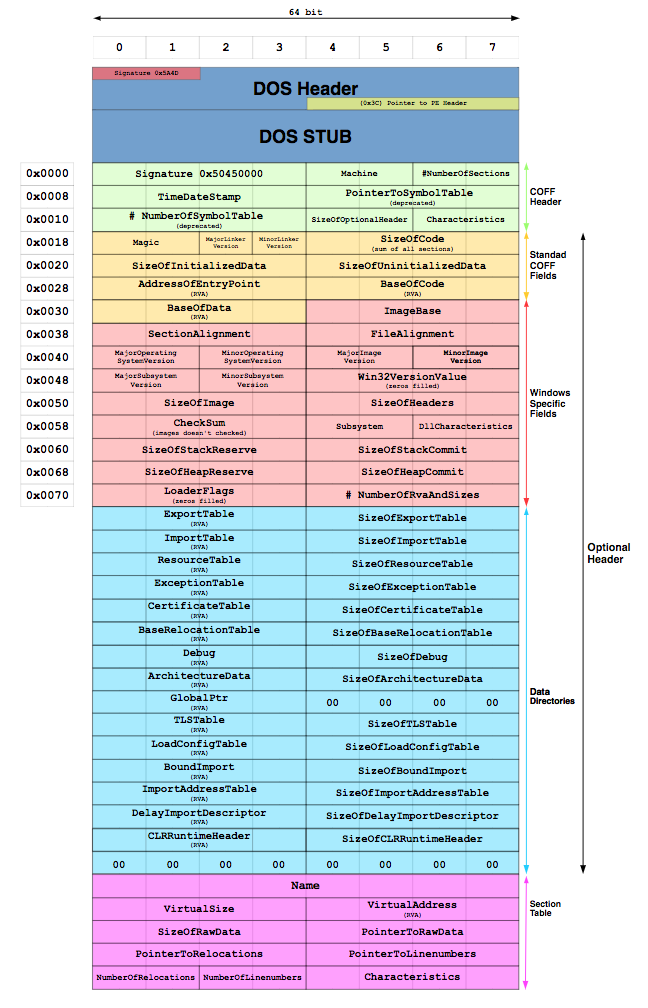
\includegraphics[width=3.6in]{figs/PEHeader.png}
    \caption{The 32-bit PE file structure. Creative commons image courtesy \cite{PEformat}.}
    \label{fig:pe_header}
\end{figure}

\subsection{PE File Format} 
\label{sec:pe}
The PE file format describes the predominant executable format for Microsoft Windows operating systems, and includes executables, dynamically-linked libraries (DLLs), and FON font files. The format is currently supported on Intel, AMD and variants of ARM instruction set architectures.

The file format is arranged with a number of standard headers (see Fig. \ref{fig:pe_header} for PE-32 format), followed by one or more sections \cite{pietrek2002inside}.  Headers include the Common Object File Format (COFF) file header that contains important information such as the type of machine for which the file is intended, the nature of the file (DLL, EXE, OBJ), the number of sections, the number of symbols, etc.  The optional header identifies the linker version, the size of the code, the size of initialized and uninitialized data, the address of the entry point, etc.  Data directories within the optional header provide pointers to the sections that follow it.  This includes tables for exports, imports, resources, exceptions, debug information, certificate information, and relocation tables.  As such, it provides a useful summary of the contents of an executable \cite{shafiq2009pe}. Finally, the section table outlines the name, offset and size of each section in the PE file.

PE sections contain code and initialized data that the Windows loader is to map into executable or readable/writeable memory pages, respectively, as well as imports, exports and resources defined by the file.  Each section contains a header that specifies the size and address.  An import address table instructs the loader which functions to statically import.  A resources section may contain resources such as required for user interfaces: cursors, fonts, bitmaps, icons, menus, etc.  A basic PE file would normally contain a \texttt{.text} code section and one or more data sections (\texttt{.data}, \texttt{.rdata} or \texttt{.bss}).  Relocation tables are typically stored in a \text{.reloc} section, used by the Windows loader to reassign a base address from the executable's preferred base.  A \texttt{.tls} section contains special thread local storage (TLS) structure for storing thread-specific local variables, which has been exploited to redirect the entry point of an executable to first check if a debugger or other analysis tool are being run \cite{brand2010malware}.  Section names are arbitrary from the perspective of the Windows loader, but specific names have been adopted by precedent and are overwhelmingly common.  Packers may create new sections, for example, the UPX packer creates \texttt{UPX1} to house packed data and an empty section \texttt{UPX0} that reserves an address range for runtime unpacking \cite{devi2012pe}.
\pagebreak[3]

\subsection{Static PE Malware Detection} \label{sec:staticpe}
Static malware detection attempts to classify samples as malicious or benign without executing them, in contrast to dynamic malware detection which detects malware based on its runtime behavior including time-dependent sequences of system calls for analysis~\cite{dahl2013large,pascanu2015malware,athiwaratkun2017malware}. Although static detection is well-known to be undecidable in general~\cite{cohen1987computer}, it is an important protection layer in a security suite because when successful, it allows malicious files to be detected prior to execution. 

Machine learning-based static PE malware detectors have been used since at least 2001~\cite{schultz2001data}, and owing largely to the structured file format and backwards-compatibility requirements, many concepts remain surprisingly similar in subsequent works~\cite{kolter2004learning, shafiq2009framework, raman2012selecting, dahl2013large, saxe2015deep}.  Schultz et al.~\cite{schultz2001data} assembled a dataset and generated labels by running through a McAfee virus scanner.  PE files were represented by features that included imported functions, strings and byte sequences.  Various machine learning models were trained and validated on a holdout set. Models included rules induced from RIPPER~\cite{cohen1995fast}, na\"{i}ve Bayes and an ensemble classifier. Kolter et al.~\cite{kolter2004learning} extended this approach by including byte-level N-grams, and employed techniques from natural language processing, including tf-idf weighting of strings.  Shafiq et al.~\cite{shafiq2009framework} proposed using just seven features from the PE header (described in Section \ref{sec:datasets}), motivated by the fact that most malware samples in their study typically exhibited those elements.  Saxe and Berlin leveraged novel two dimensional byte entropy histograms that is fed into a multi-layer neural network for classification~\cite{saxe2015deep}.  

Recent advances in end-to-end deep learning have dramatically improved the state of the art especially in object classification, machine translation and speech recognition.  In many of these approaches, raw images, text or speech waveforms are used as input to a machine learning model which infers the most useful feature representation for the task at hand.  However, despite successes in other domains hand-crafted features apparently still represent the state of the art for malware detection in published literature.  The state of the art may change to end-to-end deep learning in the ensuing months or years, but hand-crafted features derived from parsing the PE file may continue to be relevant indefinitely because of the structured format.  A recent example of end-to-end deep learning for malware classification is discussed in \cite{raff2017malware}, which we re-implement and compare to our baseline model in Section \ref{sec:results}.


\subsection{Malicious and benign datasets}
\label{sec:datasets}
PE-Miner aimed to produce a machine-learning based malware detector that exceeded 99\% true positive rate (TPR) at less than a 1\% false positive rate (FPR), with a runtime comparable to signature-based scanners of the day \cite{shafiq2009pe}.  It was trained on a dataset of $1,447$ benign files on the operating system (never published), $10,339$ malicious PE files from VX Heaven \cite{vxheaven}, and $5,586$ malicious PE files from Malfease.  PE-Miner uses 189 features that include a binary indicator for specific DLLs referenced, the sizes of various sections, summary information from the COFF section, a summary of the resource table, etc.  Unfortunately, many of the features were not disclosed publicly, some being deemed sensitive and protected under NDA \cite{seymour2016howto}.  Several model types were evaluated on the dataset, and of those, it was discovered that the J48 decision tree algorithm provided the best performance.  Notably, although many papers cite this work as one of the first performant (both speed and TP/FP rates) non-signature-based methods, the lack of public dataset has resulted no real comparative study.

Shortly following, the Adobe Malware Classifier aimed to produce a malware classifier from only seven features\footnote{The feature set we release in EMBER contains all of the information required to recreate features for the Adobe Malware Classifier.}: debug size, image version, relative virtual address of the import address table, export size, resource size, virtual size of the second section, and the total number of sections \cite{raman2012selecting}. A decision tree algorithm was trained and the resulting classifier released as a freely available tool\footnote{\url{https://sourceforge.net/adobe/malclassifier/wiki/Home/}}.  It has been suggested, however, that since the benign dataset largely comprised of Windows binaries, the resulting model is strongly biased towards a non-Windows vs. Windows rather than a malicious vs. benign problem \cite{seymour2016howto}. Indeed, in evaluating the pretrained model on the EMBER test set, we observe extremely large false positive rates and low detection rates (see Section \ref{sec:results}). Unfortunately, the dataset consisting of about 100K malicious files and 16K benign files was never released for comparative research.  

In contrast, the Microsoft Malware Classification Challenge concluded in April 2015 \cite{ronen2018microsoft}.  The dataset included a large dataset of 500MB, consisting of disassembly and bytecode of around 20K malicious samples from nine families.   The largest family consisted of features from 3K samples (\texttt{Kelihos} backdoor), while the smallest family included only 42 samples (\texttt{Simda} backdoor).  Since the conclusion of the competition, more than 50 research papers and theses cited the dataset.  A contributional summary of many of these works are tabulated in \cite{ronen2018microsoft}.  Unfortunately, the disassembly features are specific to IDA Pro disassembler (not easily reproducible), and the dataset contains no benign files.

Malware sharing services like VXHeaven provide an ample supply of malicious binaries \cite{vxheaven}.  VirusTotal can be mined for supposed benign files using heuristics about the number of detections of vendor participants \cite{virustotal}.  However, large-scale file access rates in VirusTotal require a payed subscription.  Regardless, an agreed-upon set of malicious and benign files for machine learning benchmark purposes is so far non-existent.
